\documentclass[compress,red,mathsans,10pt]{beamer}
\usepackage{beamerthemesplit}
\usepackage{amssymb}
\usepackage{multirow}
\usepackage{srcltx}
%\usetheme{Antibes}
\usepackage{pgf,pgfarrows,pgfnodes}

\setbeamercolor{uppercol}{fg=white,bg=purple}%
\setbeamercolor{lowercol}{fg=black,bg=pink}%


\usecolortheme{lily}
\begin{document}
\title{Aplicacions Estad\'{\i}stiques}
\subtitle{Enginyeria Edificaci\'o 2009/10.}  
\author{Antonio E. Teruel}
\date{}

\frame{\titlepage} 

\frame{\frametitle{Temari}
\begin{itemize}
\item  {\color{red}Estad\'{\i}stica Descriptiva\color{black}}
	\begin{itemize}
	\item [] Tema 1. \color{red}An\`alisi exploratori de dades.\color{black}
	\item [] Tema 2. Distribucions estad\'{\i}stiques bidimensionals. 
	\end{itemize}
\item Probabilitat.
	\begin{itemize}
	 \item [] Tema 3. Teoria de la probabilitat.
	\end{itemize}
\item Estad\'{\i}stica Inferencial.
	\begin{itemize}
	\item [] Tema 4. Variables aleat\`ories discretes.
	\item [] Tema 5. Variables aleat\`ories continues.
	\item [] Tema 6. Estimaci\'o de par\`ametres.
	\item [] Tema 7. Contrast d'hipòtesis.
	\end{itemize}
\end{itemize}
}

\frame{\frametitle{Representaci\'o de dades estad\'{\i}stiques}
\begin{itemize}
\item Les dades obtingudes d'un estudi estad\'{\i}stic s'anomenen dades brutes. 
\item Aquestes dades s'organitzen en taules de freq\"u\`encies.
\item[]
\end{itemize}

\begin{center}
 \begin{tabular}{|c|}\hline
$\mathbf{x}_i$\\ \hline
$x_1$\\ \hline
$x_2$\\ \hline
$x_3$\\ \hline
$\vdots$\\ \hline
$x_n$\\ \hline  
 \end{tabular}
$\Longrightarrow$
\begin{tabular}{|c|c|c|c|c|c|c|}\hline
$\mathbf{x}_i$ & $\mathbf{n}_i$ & $\mathbf{N}_i$ & $\mathbf{f}_i$ & $\mathbf{F}_i$& $\mathbf{p}_i$ & $\mathbf{P}_i$ \\ \hline
$x_1$ & $n_1$ &$N_1$ &$f_1$ &$F_1$ &$p_1$ &$P_1$ \\ \hline
$x_2$ & $n_2$ &$N_2$ &$f_2$ &$F_2$ &$p_2$ &$P_2$\\ \hline
$x_3$ & $n_3$ &$N_3$ &$f_3$ &$F_3$ &$p_3$ &$P_3$ \\ \hline
$\vdots$&$\vdots$&$\vdots$&$\vdots$&$\vdots$&$\vdots$&$\vdots$\\ \hline
$x_k$ & $n_k$ &$N_k=n$ &$f_k$ &$F_k=1$ &$p_k$ &$P_k=100$\\ \hline   
\end{tabular}
\end{center}
\begin{picture}(0,0)
\put(10,0){Dades brutes}
\put(130,0){Taula de Freq\"u\`encies}
\end{picture}
}

\frame{\frametitle{Representaci\'o de dades estad\'{\i}stiques}
\begin{itemize}
\item Les taules de freq\"u\`encia contenen informaci\'o de:
	\begin{itemize}
	\item els valors de la variable: $x_i$
	\item nombre de vegades que apareix cada valor (freq\"u\`encia absoluta): ${n}_i$
	\item el nombre total de valors: ${n}$
	\item \color{red}les freq\"u\`encies absolutes acumulades: $N_i=n_1+n_2+...+n_i$\color{black}
	\item les freq\"u\`encies relatives: $f_i=\dfrac{n_i}{n}$
	\item \color{red}les freq\"u\`encies relatives acumulades: $F_i=\dfrac{N_i}{n}$\color{black}
	\item els percentatges absoluts: $p_i= f_i x 100\%$
	\item \color{red}els percentatges acumulats: $P_i= F_i x 100\%$\color{black}
	\end{itemize}
\item []
\item En color \color{red}vermell \color{black} nom\`es per a variables quantitatives i ordinals.
\end{itemize}

}

\frame{\frametitle{Representaci\'o de dades estad\'{\i}stiques}
\vspace{1cm}
\begin{center}
 \begin{tabular}{|c|}\hline
$\mathbf{x}_i$\\ \hline
$x_1$\\ \hline
$x_2$\\ \hline
$x_3$\\ \hline
$\vdots$\\ \hline
$x_n$\\ \hline  
 \end{tabular}
$\Longrightarrow$
\begin{tabular}{|c|c|c|c|c|c|c|}\hline
$\mathbf{x}_i$ & $\mathbf{n}_i$ & $\mathbf{N}_i$ & $\mathbf{f}_i$ & $\mathbf{F}_i$& $\mathbf{p}_i$ & $\mathbf{P}_i$ \\ \hline
$x_1$ & $n_1$ &$N_1$ &$f_1$ &$F_1$ &$p_1$ &$P_1$ \\ \hline
$x_2$ & $n_2$ &$N_2$ &$f_2$ &$F_2$ &$p_2$ &$P_2$\\ \hline
$x_3$ & $n_3$ &$N_3$ &$f_3$ &$F_3$ &$p_3$ &$P_3$ \\ \hline
$\vdots$&$\vdots$&$\vdots$&$\vdots$&$\vdots$&$\vdots$&$\vdots$\\ \hline
$x_k$ & $n_k$ &$N_k=n$ &$f_k$ &$F_k=1$ &$p_k$ &$P_k=100$\\ \hline   
\end{tabular}
\end{center}
\begin{picture}(0,0)
\put(10,0){Dades brutes}
\put(130,0){Taula de Freq\"u\`encies}
\put(12,120){$n$ valors}
\put(37,117){\line(-1,0){10}\vector(0,-1){25}}
\put(65,120){$k$ valors}
\put(85,117){\line(-1,0){10}\vector(0,-1){25}}
\put(85,140){\color{red}freq.abs.acum.\color{black}}
\put(120,137){\line(1,0){10}\vector(0,-1){42}}
\put(90,110){freq.abs}
\put(105,107){\line(-1,0){10}\vector(0,-1){12}}
\put(135,110){freq.rel}
\put(150,107){\line(1,0){10}\vector(0,-1){12}}
\put(160,140){\color{red}freq.rel.acum.\color{black}}
\put(180,137){\line(1,0){10}\vector(0,-1){42}}
\put(200,110){\% abs}
\put(217,107){\line(1,0){10}\vector(0,-1){12}}
\put(230,140){\color{red}\%.abs.acum.\color{black}}
\put(250,137){\line(1,0){10}\vector(0,-1){42}}
\end{picture}
\newline\newline
En color \color{red}vermell \color{black} nom\`es per a variables quantitatives i ordinals.
}

\frame{\frametitle{Representaci\'o de dades estad\'{\i}stiques}
\begin{itemize}
\item Exemple: nota d'estad\'{\i}stica de 10 persones
\item[]
\end{itemize}

\begin{center}
 \begin{tabular}{|c|}\hline
$\mathbf{x}_i$\\ \hline
$7$\\ \hline
$5$\\ \hline
$9$\\ \hline
$7$\\ \hline
$5$\\ \hline  
$6$\\ \hline  
$7$\\ \hline  
$6$\\ \hline  
$4$\\ \hline
$7$\\ \hline  
\end{tabular}
$\Longrightarrow$
\begin{tabular}{|c|c|c|c|c|c|c|}\hline
$\mathbf{x}_i$ & $\mathbf{n}_i$ & $\mathbf{N}_i$ & $\mathbf{f}_i$ & $\mathbf{F}_i$& $\mathbf{p}_i$ & $\mathbf{P}_i$ \\ \hline
$4$ & $1$ &$1$ &$0.1$ &$0.1$ &$10$ &$10$ \\ \hline
$5$ & $2$ &$3$ &$0.2$ &$0.3$ &$20$ &$30$\\ \hline
$6$ & $2$ &$5$ &$0.2$ &$0.5$ &$20$ &$50$ \\ \hline
$7$ & $4$ &$9$ &$0.4$ &$0.9$ &$40$ &$90$ \\ \hline
$9$ & $1$ &$10$ &$0.1$ &$1.0$ &$10$ &$100$ \\ \hline
\end{tabular}
\end{center}
\begin{picture}(0,0)
\put(35,0){Dades brutes}
\put(130,0){Taula de Freq\"u\`encies}
\put(115,25){$n=10$}
\put(160,25){$f=1$}
\end{picture}
}

\frame{\frametitle{Representaci\'o de dades estad\'{\i}stiques amb intervals}

\begin{itemize}
\item Representaci\'o de dades amb intervals
	\begin{itemize}
	\item nom\'es variables quantitatives i qualitatives ordinals
	\item s'agrupen en intervals de valors
	\item s'anomena marca de classe $(m)$ al valor representatiu d'un interval i \'es igual al valor mitj\`a de l'interval
	\end{itemize}
\end{itemize}
}

\frame{\frametitle{Representaci\'o de dades estad\'{\i}stiques}
\begin{itemize}
\item Exemple: nota d'estad\'{\i}stica de 20 persones
\item[]
\end{itemize}

\begin{center}
 \begin{tabular}{|c|c|c|}  \cline{1-1} \cline{3-3}
$8.4$ & & $9.4$ \\  \cline{1-1} \cline{3-3} 
$5.5$ & & $7.5$\\  \cline{1-1} \cline{3-3} 
$9.1$ & & $8.1$\\  \cline{1-1} \cline{3-3} 
$6.9$ & & $5.7$\\   \cline{1-1} \cline{3-3}
$5.3$ & & $6.4$\\    \cline{1-1} \cline{3-3}
$6.2$ & & $5.8$\\   \cline{1-1} \cline{3-3}
$7.8$ & & $4.8$\\  \cline{1-1} \cline{3-3} 
$6.1$ & & $6.0$\\   \cline{1-1} \cline{3-3} 
$4.2$ & & $4.7$\\  \cline{1-1} \cline{3-3} 
$3.9$ & & $7.9$\\  \cline{1-1} \cline{3-3} 
\end{tabular}
$\Longrightarrow$
\begin{tabular}{|c|c|c|c|c|c|c|c|}\hline
$\mathbf{x}_i$ & $\mathbf{m}_i$ & $\mathbf{n}_i$ & $\mathbf{N}_i$ & $\mathbf{f}_i$ & $\mathbf{F}_i$& $\mathbf{p}_i$ & $\mathbf{P}_i$ \\ \hline
$[0,4)$& $2$   &$1$&$1$ &$0.05$ &$0.05$&$5$ &$5$ \\ \hline
$[4,5)$& $4.5$ &$3$&$4$ &$0.15$ &$0.20$&$15$ &$20$\\ \hline
$[5,7)$& $6$   &$9$&$13$&$0.45$ &$0.65$&$45$ &$65$ \\ \hline
$[7,9)$& $8$   &$5$&$18$&$0.25$ &$0.90$&$25$ &$90$ \\ \hline
$[9,10)$& $9.5$&$2$&$20$&$0.10$ &$1.00$&$10$ &$100$ \\ \hline
\end{tabular}
\end{center}
\begin{picture}(0,0)
\put(10,0){Dades brutes}
\put(150,0){Taula de Freq\"u\`encies}
\put(150,25){$n=20$}
\put(200,25){$f=1$}
\end{picture}
}


\frame{\frametitle{Representaci\'o gr\`afica de dades estad\'{\i}stiques}
\begin{center}
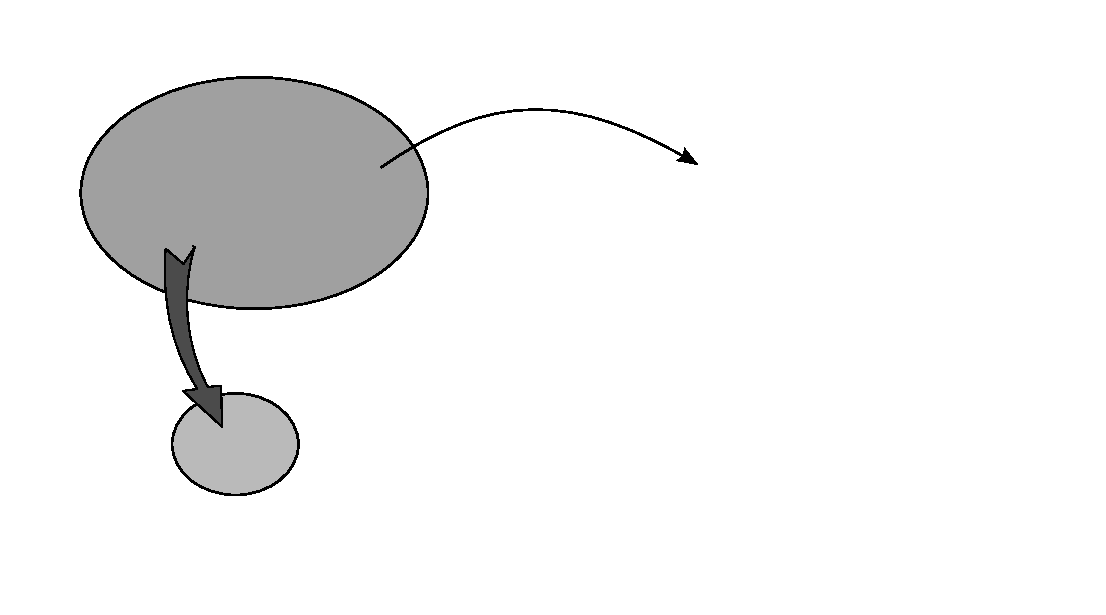
\includegraphics[width=7cm]{Dbes0103.eps}
\end{center}
\begin{picture}(0,0)
\put(170,110){Diagrama de tarta}
\put(160,10){\color{red}Pol\'{\i}gono de Freq\"u\`encies\color{black}}
\put(55,110){Diagrama de Barres}
\put(75,10){\color{red}Histograma\color{black}}
\end{picture}
\newline
En color \color{red}vermell \color{black} nom\`es per a variables quantitatives
}

\frame{\frametitle{Representaci\'o gr\`afica de dades estad\'{\i}stiques}
\begin{itemize}
\item  Diagrama de barres:
	\begin{itemize}
	\item Una barra per a cada valor o interval de valors
	\item Al\c{c}ada de les barres proporcional a la freq\"u\`encia (absoluta o relativa)
	\end{itemize}
\item Exemple:
\end{itemize}
\begin{columns}
\begin{column}{0.5\textwidth}
\begin{tabular}{|c|c|c|c|c|c|c|}\hline
$\mathbf{x}_i$ & $\mathbf{n}_i$ & $\mathbf{N}_i$ & $\mathbf{f}_i$ & $\mathbf{F}_i$& $\mathbf{p}_i$ & $\mathbf{P}_i$ \\ \hline
$4$ & $1$ &$1$ &$0.1$ &$0.1$ &$10$ &$10$ \\ \hline
$5$ & $2$ &$3$ &$0.2$ &$0.3$ &$20$ &$30$\\ \hline
$6$ & $2$ &$5$ &$0.2$ &$0.5$ &$20$ &$50$ \\ \hline
$7$ & $4$ &$9$ &$0.4$ &$0.9$ &$40$ &$90$ \\ \hline
$9$ & $1$ &$10$ &$0.1$ &$1.0$ &$10$ &$100$ \\ \hline
\end{tabular}
\end{column}
\begin{column}{0.5\textwidth}
\begin{center}
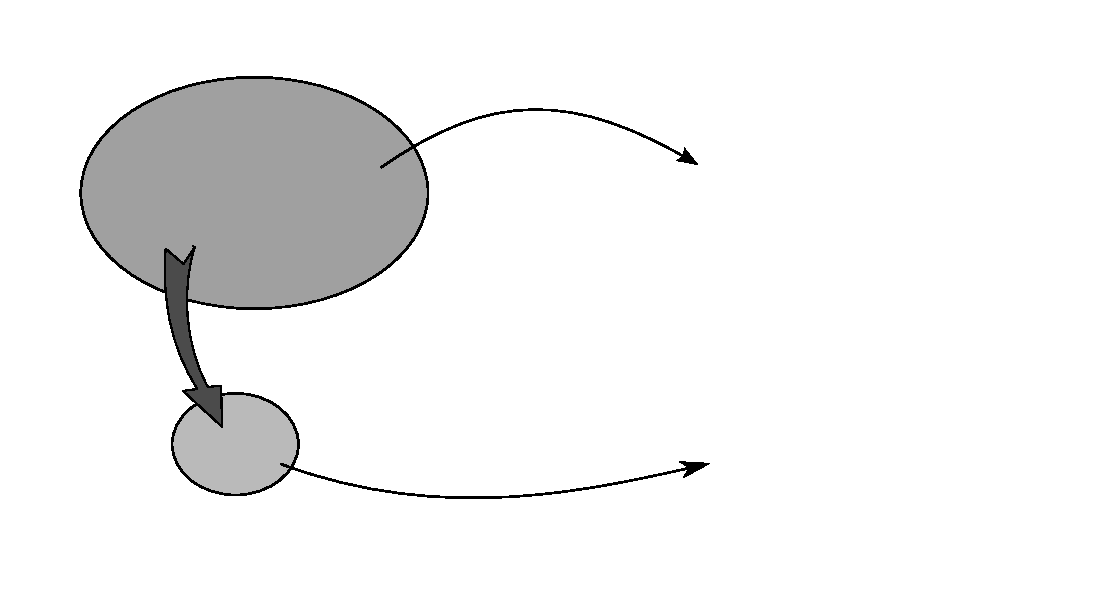
\includegraphics[width=3cm]{Dbes0104.eps}
\put(-100,125){$\mathbf{n}_i$}
\put(-100,50){$\mathbf{N}_i$}
\end{center}
\end{column}
\end{columns}
}

\frame{\frametitle{Representaci\'o gr\`afica de dades estad\'{\i}stiques}
\begin{itemize}
\item  Diagrama de tarta:
	\begin{itemize}
	\item Un sector per a cada valor o interval de valors
	\item \`Area del sector proporcional a la freq\"u\`encia (absoluta o relativa)
	\end{itemize}
\item Exemple:
\end{itemize}
\begin{columns}
\begin{column}{0.5\textwidth}
\begin{tabular}{|c|c|c|c|c|c|c|}\hline
$\mathbf{x}_i$ & $\mathbf{n}_i$ & $\mathbf{N}_i$ & $\mathbf{f}_i$ & $\mathbf{F}_i$& $\mathbf{p}_i$ & $\mathbf{P}_i$ \\ \hline
$4$ & $1$ &$1$ &$0.1$ &$0.1$ &$10$ &$10$ \\ \hline
$5$ & $2$ &$3$ &$0.2$ &$0.3$ &$20$ &$30$\\ \hline
$6$ & $2$ &$5$ &$0.2$ &$0.5$ &$20$ &$50$ \\ \hline
$7$ & $4$ &$9$ &$0.4$ &$0.9$ &$40$ &$90$ \\ \hline
$9$ & $1$ &$10$ &$0.1$ &$1.0$ &$10$ &$100$ \\ \hline
\end{tabular}
\end{column}
\begin{column}{0.5\textwidth}
\begin{center}
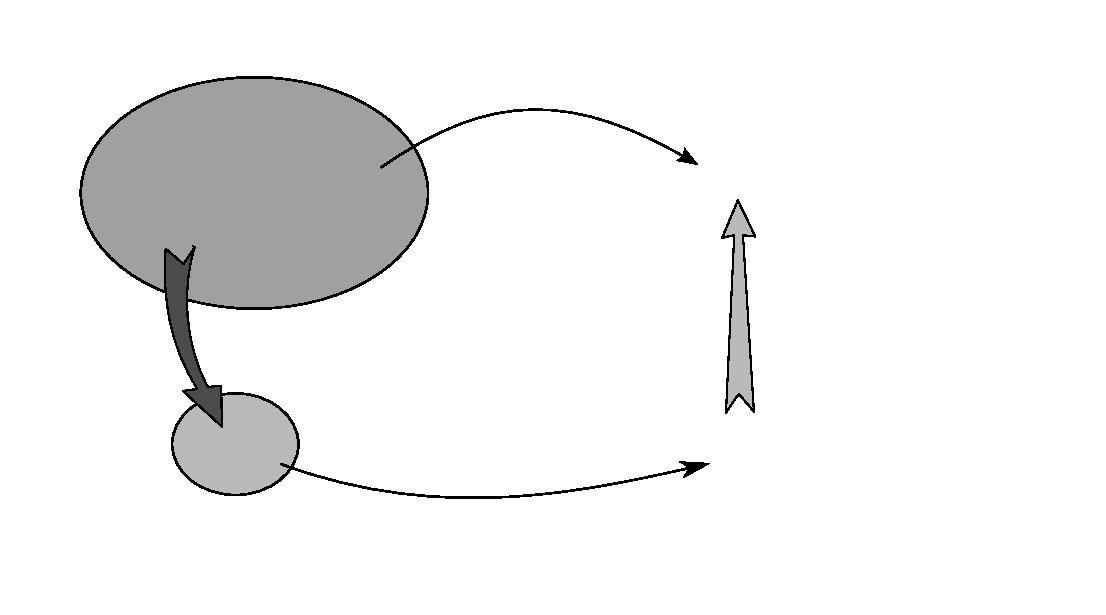
\includegraphics[width=5cm]{Dbes0105.eps}
\put(-50,125){$\mathbf{p}_i$}
\end{center}
\end{column}
\end{columns}
}

\frame{\frametitle{Representaci\'o gr\`afica de dades estad\'{\i}stiques}
\begin{itemize}
\item  Histograma:
	\begin{itemize}
	\item Una barra per a cada interval de valors
	\item Intervals de valors consecutius i sense espai entre barres (nom\'es variables quantitatives continues)
	\item \`Area de la barra (no altura) proporcional a la freq\"u\`encia (absoluta o relativa)  (histograma de densitats)
	\end{itemize}
\item Exemple:
\end{itemize}
\begin{columns}
\begin{column}{0.7\textwidth}
\begin{tabular}{|c|c|c|c|c|c|c|c|}\hline
$\mathbf{x}_i$ & $\mathbf{m}_i$ & $\mathbf{n}_i$ & $\mathbf{N}_i$ & $\mathbf{f}_i$ & $\mathbf{F}_i$& $\mathbf{p}_i$ & $\mathbf{P}_i$ \\ \hline
$[0,4)$& $2$   &$1$&$1$ &$0.05$ &$0.05$&$5$ &$5$ \\ \hline
$[4,5)$& $4.5$ &$3$&$4$ &$0.15$ &$0.20$&$15$ &$20$\\ \hline
$[5,7)$& $6$   &$9$&$13$&$0.45$ &$0.65$&$45$ &$65$ \\ \hline
$[7,9)$& $8$   &$5$&$18$&$0.25$ &$0.90$&$25$ &$90$ \\ \hline
$[9,10)$& $9.5$&$2$&$20$&$0.10$ &$1.00$&$10$ &$100$ \\ \hline
\end{tabular}
\end{column}
\begin{column}{0.4\textwidth}
\begin{itemize}
\item[] 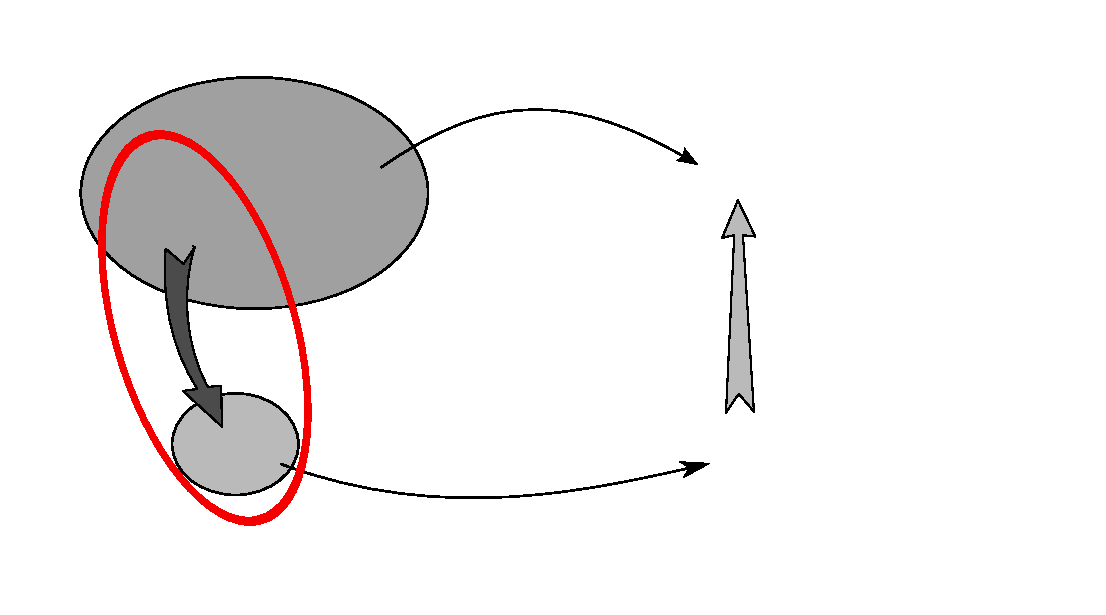
\includegraphics[width=3.5cm]{Dbes0106.eps}
% \begin{picture}
\put(-50,85){$\mathbf{n}_i$} 
% \end{picture}
\item[]
\end{itemize}
\end{column}
\end{columns}
}


\frame{\frametitle{Representaci\'o gr\`afica de dades estad\'{\i}stiques}
\begin{itemize}
\item  Pol\'{\i}gon de freq\"u\`encies:
	\begin{itemize}
	\item A partir de l'histograma
	\item L\'{\i}nees que uneixen els centres del intervals
	\item[]
	\end{itemize}
\item Exemple:
\end{itemize}
\begin{columns}
\begin{column}{0.7\textwidth}
\begin{tabular}{|c|c|c|c|c|c|c|c|}\hline
$\mathbf{x}_i$ & $\mathbf{m}_i$ & $\mathbf{n}_i$ & $\mathbf{N}_i$ & $\mathbf{f}_i$ & $\mathbf{F}_i$& $\mathbf{p}_i$ & $\mathbf{P}_i$ \\ \hline
$[0,4)$& $2$   &$1$&$1$ &$0.05$ &$0.05$&$5$ &$5$ \\ \hline
$[4,5)$& $4.5$ &$3$&$4$ &$0.15$ &$0.20$&$15$ &$20$\\ \hline
$[5,7)$& $6$   &$9$&$13$&$0.45$ &$0.65$&$45$ &$65$ \\ \hline
$[7,9)$& $8$   &$5$&$18$&$0.25$ &$0.90$&$25$ &$90$ \\ \hline
$[9,10)$& $9.5$&$2$&$20$&$0.10$ &$1.00$&$10$ &$100$ \\ \hline
\end{tabular}
\end{column}
\begin{column}{0.4\textwidth}
\begin{itemize}
\item[] 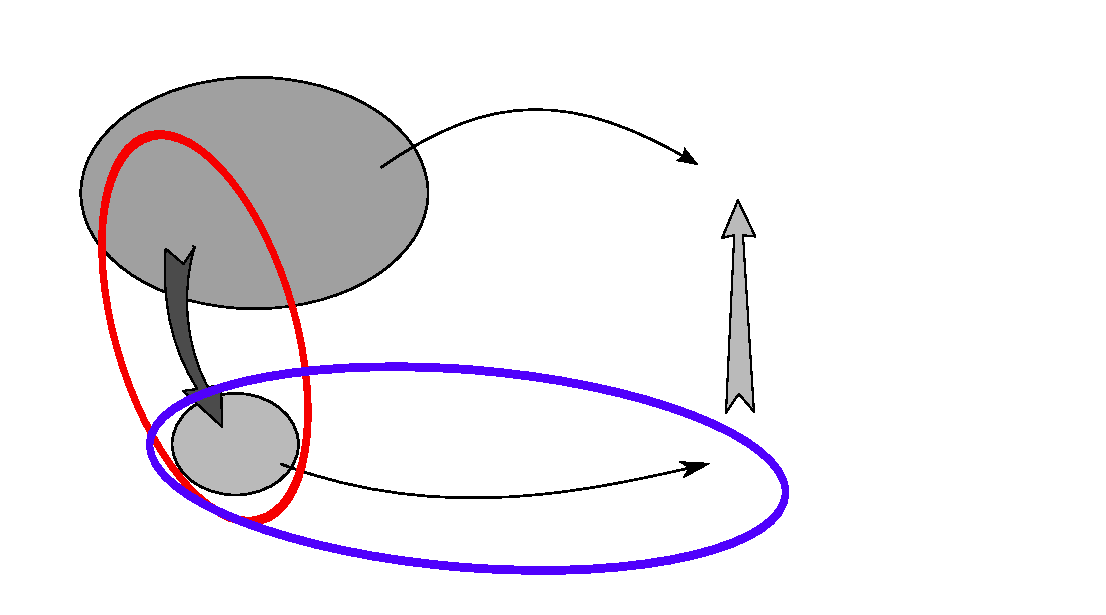
\includegraphics[width=3.5cm]{Dbes0107.eps}
% \begin{picture}
\put(-50,85){$\mathbf{n}_i$} 
% \end{picture}
\item[]
\end{itemize}
\end{column}
\end{columns}
}


\end{document}